\documentclass[]{beamer}

\usepackage[english]{babel}
\usepackage[utf8]{inputenc}
\usepackage[T1]{fontenc}
\usepackage{comment}
\usepackage{booktabs}
\usepackage{multicol}
\usepackage{changepage}
\usetheme[
  workplace=fi,
]{MU}

\graphicspath{{../}}

\definecolor{urlcolor}{RGB}{6, 69, 173}
\definecolor{imageBorderColor}{RGB}{91, 91, 91}

\fboxsep=0pt
\fboxrule=1pt

\newcommand{\TODO}{\textbf{\textcolor{red}{TODO}}} % red bold TODO

\begin{document}

\setbeamertemplate{frametitle}[default][center]
\setlength\columnsep{10pt}

\title[PA181]{PA181}
\subtitle[Term Project]{Term Project}
\author[A.\,Tóth, J.\,Ondruch, J.\,Čechák, T.\,Pavlík, V.\,Stehlík]{
  \begin{scriptsize}
    \begin{tabular}{r@{\hspace{2mm}}l}
      Adrián Tóth    & {\normalfont \href{mailto:491322@mail.muni.cz}{\color{urlcolor}{491322@mail.muni.cz}}}\\[1mm]
      Jiří Čechák    & {\normalfont \href{mailto:445717@mail.muni.cz}{\color{urlcolor}{445717@mail.muni.cz}}}\\[1mm]
      Jan Ondruch    & {\normalfont \href{mailto:433341@mail.muni.cz}{\color{urlcolor}{433341@mail.muni.cz}}}\\[1mm]
      Tadeáš Pavlík  & {\normalfont \href{mailto:487555@mail.muni.cz}{\color{urlcolor}{487555@mail.muni.cz}}}\\[1mm]
      Václav Stehlík & {\normalfont \href{mailto:487580@mail.muni.cz}{\color{urlcolor}{487580@mail.muni.cz}}}\\[1mm]
    \end{tabular}
  \end{scriptsize}
}
\institute[FI MU]{Faculty of Informatics, Masaryk University}
\date{\today}
\subject{Presentation Subject}
\keywords{the, presentation, keywords}

\begin{frame}[plain]
  \begin{center}
    \maketitle
  \end{center}
\end{frame}

\begin{frame}{Table of Contents}
  \setlength{\columnsep}{-25mm}
  \begin{adjustwidth}{10mm}{-10mm}
    \begin{multicols}{2}
      \tableofcontents

      \columnbreak
      \hfill\\[7mm]
      \begin{figure}[H]
        
\includegraphics[width=.35\textwidth,height=.35\textheight,keepaspectratio]{img/content.pdf}
      \end{figure}
    \end{multicols}
  \end{adjustwidth}
\end{frame}

%##############################################################################

\section[Introduction]{Introduction}

  \subsection{About}

    \begin{frame}{About}
      \setlength{\columnsep}{-125mm}
      \begin{adjustwidth}{20mm}{-25mm}
        \begin{multicols}{2}
          \begin{itemize}
            \item term project
            \item team project
            \item cloud native
            \item something useful
          \end{itemize}

          \columnbreak

          \begin{figure}[H]
            
\includegraphics[width=.25\textwidth,height=.25\textheight,keepaspectratio]{img/info.pdf}
          \end{figure}
        \end{multicols}
      \end{adjustwidth}
    \end{frame}

  \subsection{Idea}

    \begin{frame}{Idea}
      \begin{multicols}{2}
        \begin{itemize}
          \item system for user self-testing
          \item users are able to test themselves
          \item users can add new tests
          \item multilingual
          \item good for exams preparation
        \end{itemize}

        \columnbreak

        \begin{figure}[H]
          
\includegraphics[width=.35\textwidth,height=.35\textheight,keepaspectratio]{img/idea.pdf}
        \end{figure}
      \end{multicols}
    \end{frame}

\section[Development]{Development}

  \subsection{Work Division}

    \begin{frame}{Work Division}
      \begin{adjustwidth}{-1mm}{-1mm}
        \begin{multicols}{3}
          \begin{itemize}
            \item Jan Ondruch
            \begin{itemize}
              \item specifications
              \item design
              \item testing
            \end{itemize}

            \columnbreak

            \item Jiří Čechák\\[1mm]
            \begin{itemize}
              \item design
              \item frontend
              \item testing
              \item bug fixing
            \end{itemize}

            \columnbreak

            \item Tadeáš Pavlík
            \begin{itemize}
              \item analysis
              \item design
              \item testing
            \end{itemize}
          \end{itemize}
        \end{multicols}
      \end{adjustwidth}
    \end{frame}

    \begin{frame}{Work Division}
      \setlength{\columnsep}{-20mm}
      \begin{adjustwidth}{10mm}{-10mm}
        \begin{multicols}{2}
          \begin{itemize}
            \item Adrián Tóth
            \begin{itemize}
              \item configuration
              \item architecture
              \item deployment
              \item documentation
              \item presentation
            \end{itemize}

            \columnbreak

            \item Václav Stehlík
            \begin{itemize}
              \item backend
              \item interconnection of\\backend \& frontend
              \item troubleshooting
              \item bug fixing
            \end{itemize}
          \end{itemize}
        \end{multicols}
      \end{adjustwidth}
    \end{frame}

  \subsection{Used Tools \& Technologies}

    \begin{frame}{Used Tools \& Technologies}
      \setlength{\columnsep}{-40mm}
      \begin{adjustwidth}{12.5mm}{-12.5mm}
        \begin{multicols}{2}
          Technologies:
          \begin{itemize}
            \item IBM Cloud
            \item GitHub
            \item Travis CI
          \end{itemize}

          \columnbreak

          Tools:
          \begin{itemize}
            \item IBM Cloud DevOps Toolchain
            \item ASP.NET
            \item React
            \item Material-UI
          \end{itemize}
        \end{multicols}
      \end{adjustwidth}
    \end{frame}

  \subsection{Application Initialization}

    \begin{frame}{Application Initialization}
      \begin{itemize}
        \item created one private repository
        \begin{itemize}
          \item hosted on GitHub
        \end{itemize}
        \item inspirited by IBM ASP.NET \textit{'HelloWorld'}\footnote{\href{https://github.com/IBM-Cloud/aspnet-core-helloworld}{\color{urlcolor}{github.com/IBM-Cloud/aspnet-core-helloworld}}}
        \item created project skeleton
        \begin{itemize}
          \item ASP.NET Core Web API (\textit{webapi}) - the main structure
          \item Class library (\textit{classlib}) - several support projects
        \end{itemize}
        \item configured deployment
        \begin{itemize}
          \item before the development itself
          \item on a clean \textit{'HelloWorld'} application
        \end{itemize}
        \item configured automation pipeline
        \begin{itemize}
          \item IBM Cloud DevOps Toolchain
        \end{itemize}
      \end{itemize}
    \end{frame}

  \subsection{Application Implementation}

    \begin{frame}{Application Implementation}
       \setlength{\columnsep}{-10mm}
      \begin{adjustwidth}{7mm}{-8mm}
        \begin{multicols}{2}
          Frontend:
          \begin{itemize}
            \item Material UI components
            \item connected to the API
            \item supporting any mode
            \begin{itemize}
              \item phone
              \item tablet
              \item desktop
            \end{itemize}
          \end{itemize}

          \columnbreak

          Backend:
          \begin{itemize}
            \item Model--View--Controller
            \item multitier architecture
            \begin{itemize}
              \item API
              \item entities
              \item repositories
              \item services
            \end{itemize}
          \end{itemize}
        \end{multicols}
      \end{adjustwidth}
    \end{frame}

  \subsection{Application Deployment}
    \begin{frame}{Application Deployment}
      \begin{multicols}{2}
        Our work looked like this:
        \begin{itemize}
          \item Manual
          \begin{enumerate}
            \item[1] Change code in a local repository
            \item[2] Commit changes in the local repository
            \item[3] Update of the remote repository
          \end{enumerate}
          \item Automated
          \begin{enumerate}
            \item[4] Test the application
            \item[5] Build the application from source
            \item[6] Deploy the built application
            \item[7] Create a release
          \end{enumerate}
        \end{itemize}

        \columnbreak

      \begin{figure}[H]
        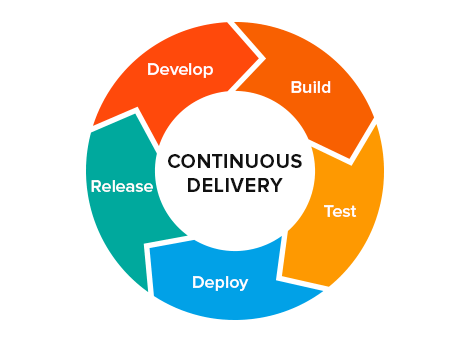
\includegraphics[width=.5\textwidth,height=.5\textheight,keepaspectratio]{img/continuous_delivery.png}
        \caption{Continuous Delivery}
      \end{figure}
      \end{multicols}
    \end{frame}

    \begin{frame}{Toolchain}
      \begin{figure}[H]
        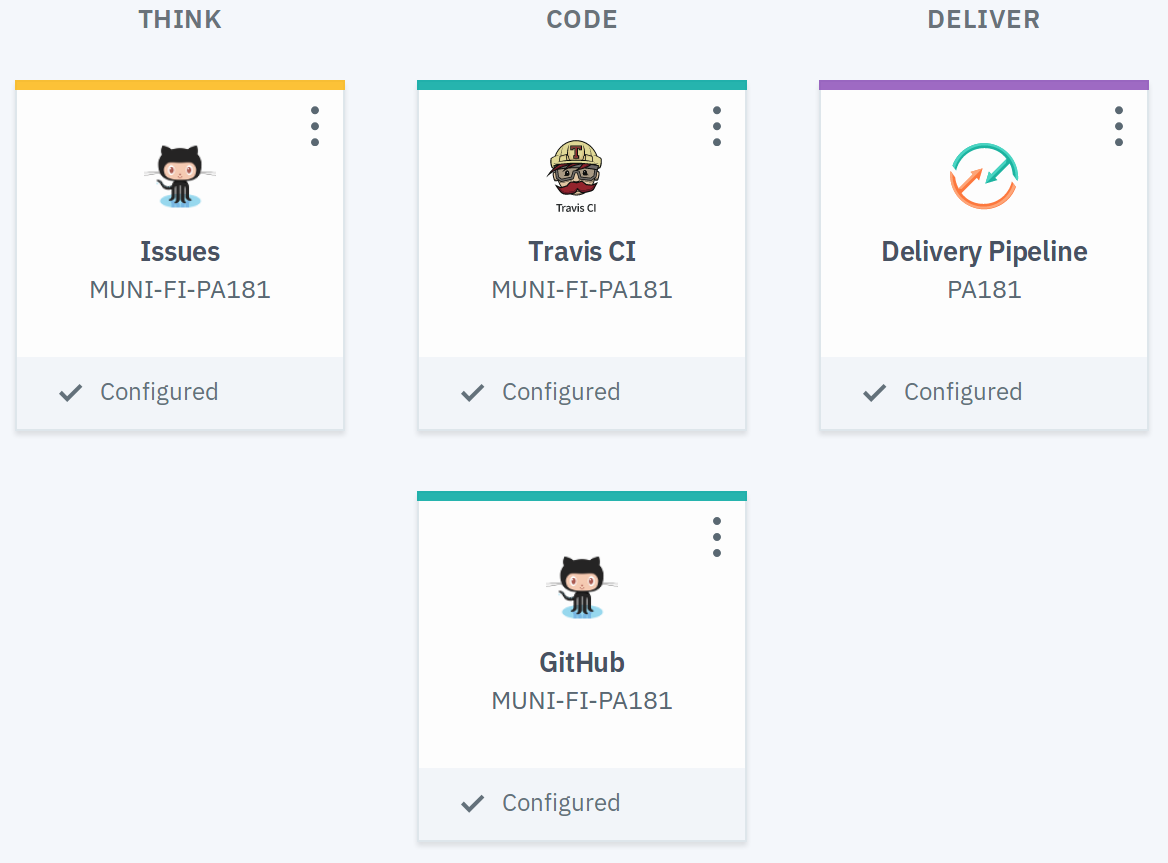
\includegraphics[width=.75\textwidth,height=.75\textheight,keepaspectratio]{img/toolchain.png}
        \caption{IBM Cloud DevOps Toolchain}
      \end{figure}
    \end{frame}

\section[Application]{Application}

  \subsection{Examples}

    \begin{frame}{Examples}
      \vspace{7.5mm}
      \centerline{The following screenshots illustrate our application.}
    \end{frame}

    \begin{frame}{Example 1}
      \begin{figure}
        \fcolorbox{imageBorderColor}{white}{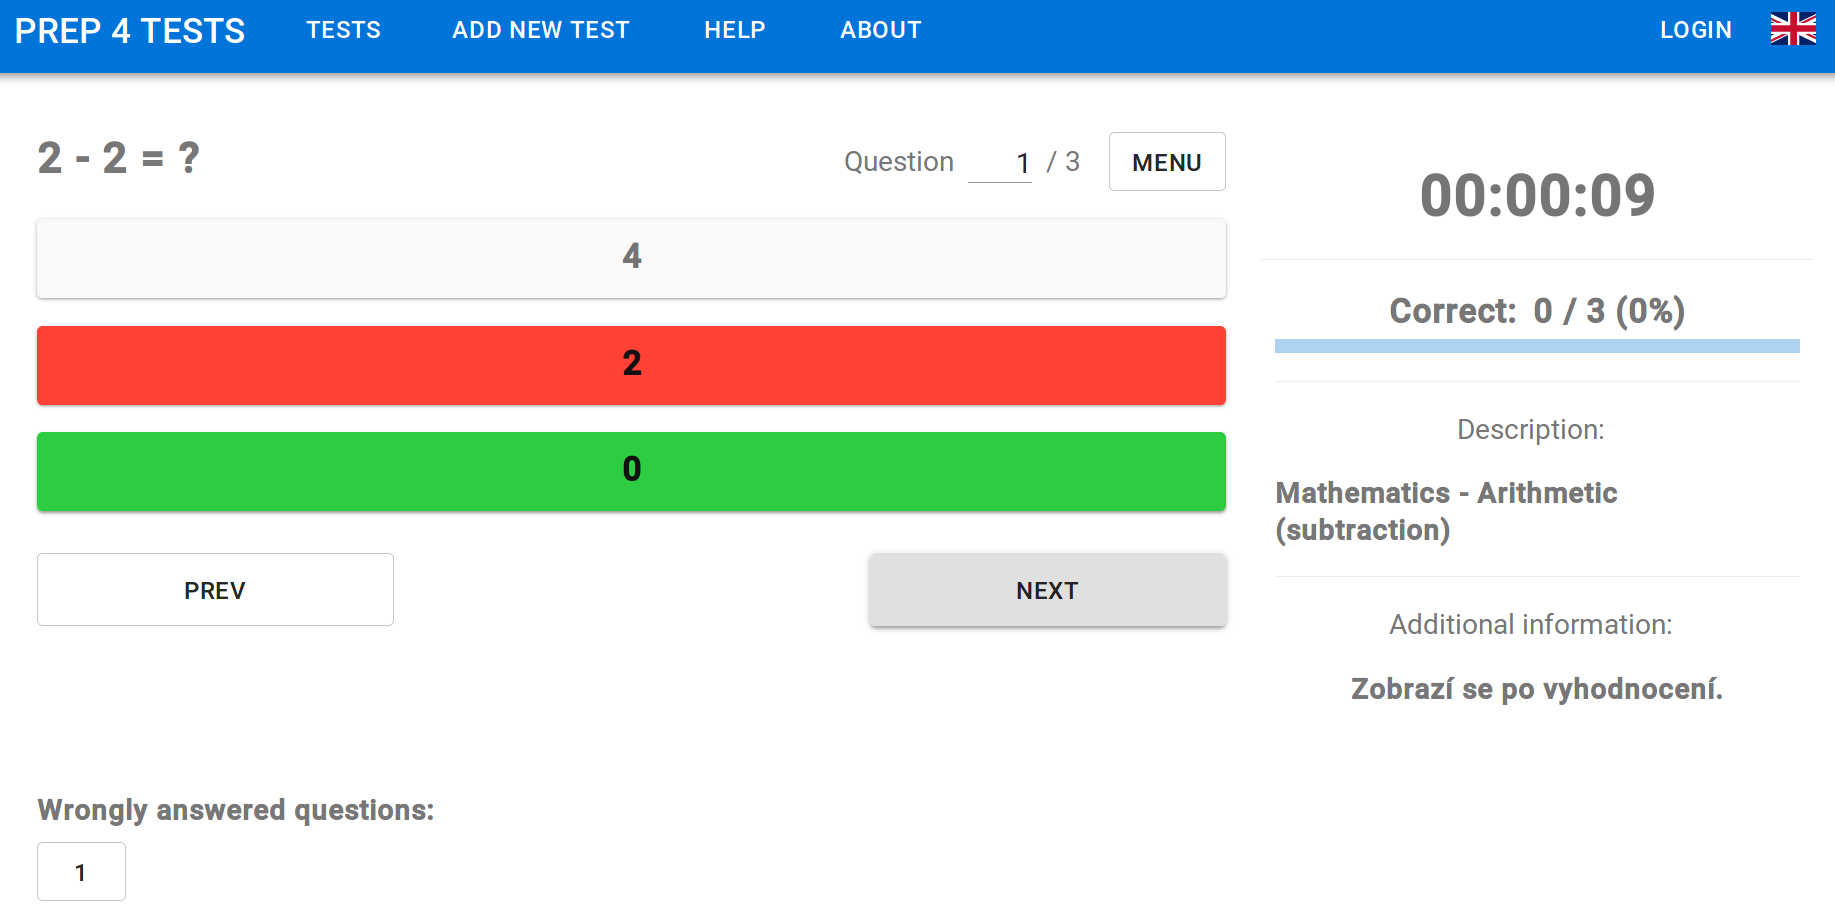
\includegraphics[width=0.75\textwidth,height=0.75\textheight,keepaspectratio]{img/application/example1.png}}
        \caption{list of available tests}
      \end{figure}
    \end{frame}

    \begin{frame}{Example 2}
      \begin{figure}
        \fcolorbox{imageBorderColor}{white}{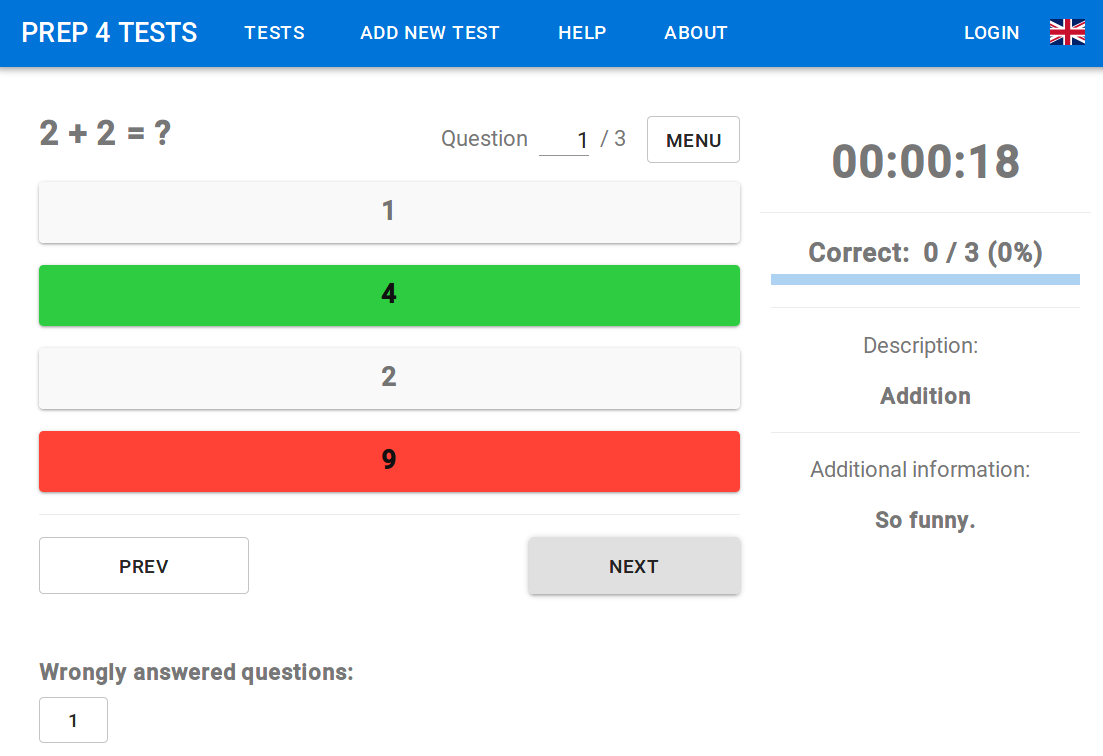
\includegraphics[width=0.8\textwidth,height=0.8\textheight,keepaspectratio]{img/application/example2.png}}
        \caption{incorrect answer}
      \end{figure}
    \end{frame}

    \begin{frame}{Example 3}
      \begin{figure}
        \fcolorbox{imageBorderColor}{white}{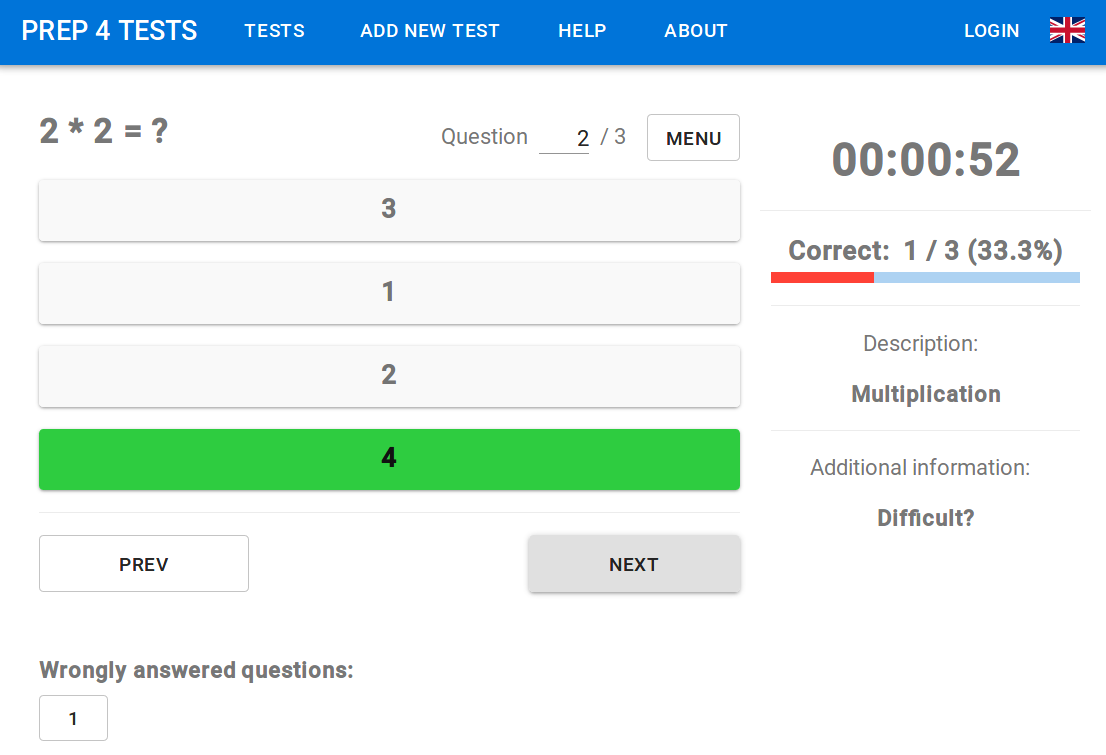
\includegraphics[width=0.8\textwidth,height=0.8\textheight,keepaspectratio]{img/application/example3.png}}
        \caption{correct answer}
      \end{figure}
    \end{frame}

    \begin{frame}{Example 4}
      \begin{figure}
        \fcolorbox{imageBorderColor}{white}{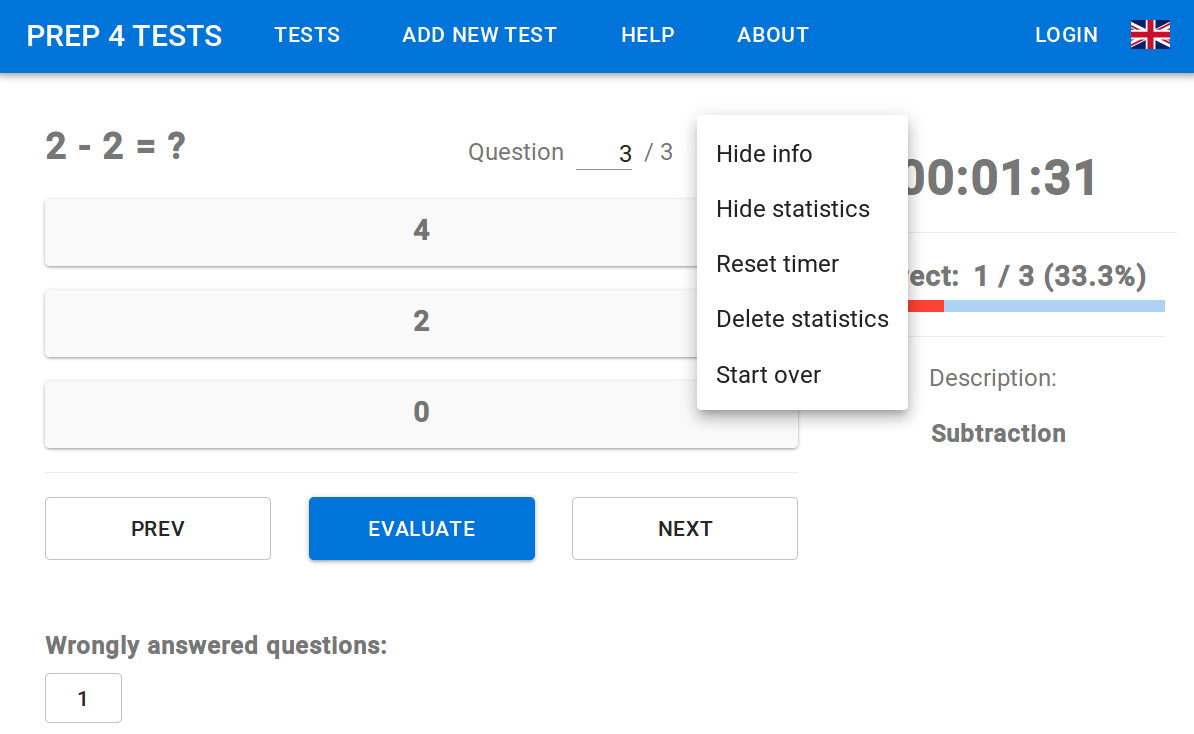
\includegraphics[width=0.8\textwidth,height=0.8\textheight,keepaspectratio]{img/application/example9.png}}
        \caption{dropdown menu}
      \end{figure}
    \end{frame}

    \begin{frame}{Example 5}
      \begin{figure}
        \fcolorbox{imageBorderColor}{white}{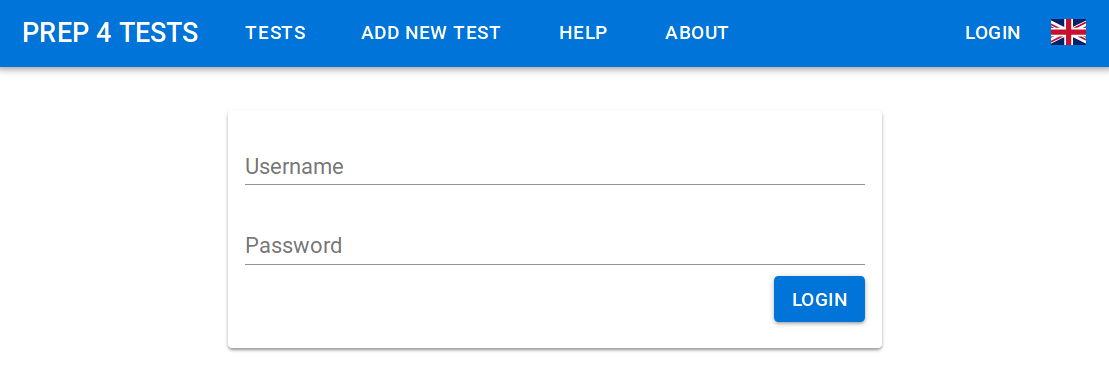
\includegraphics[width=\textwidth,height=\textheight,keepaspectratio]{img/application/example4.png}}
        \caption{login}
      \end{figure}
    \end{frame}

    \begin{frame}{Example 6}
      \begin{figure}
        \fcolorbox{imageBorderColor}{white}{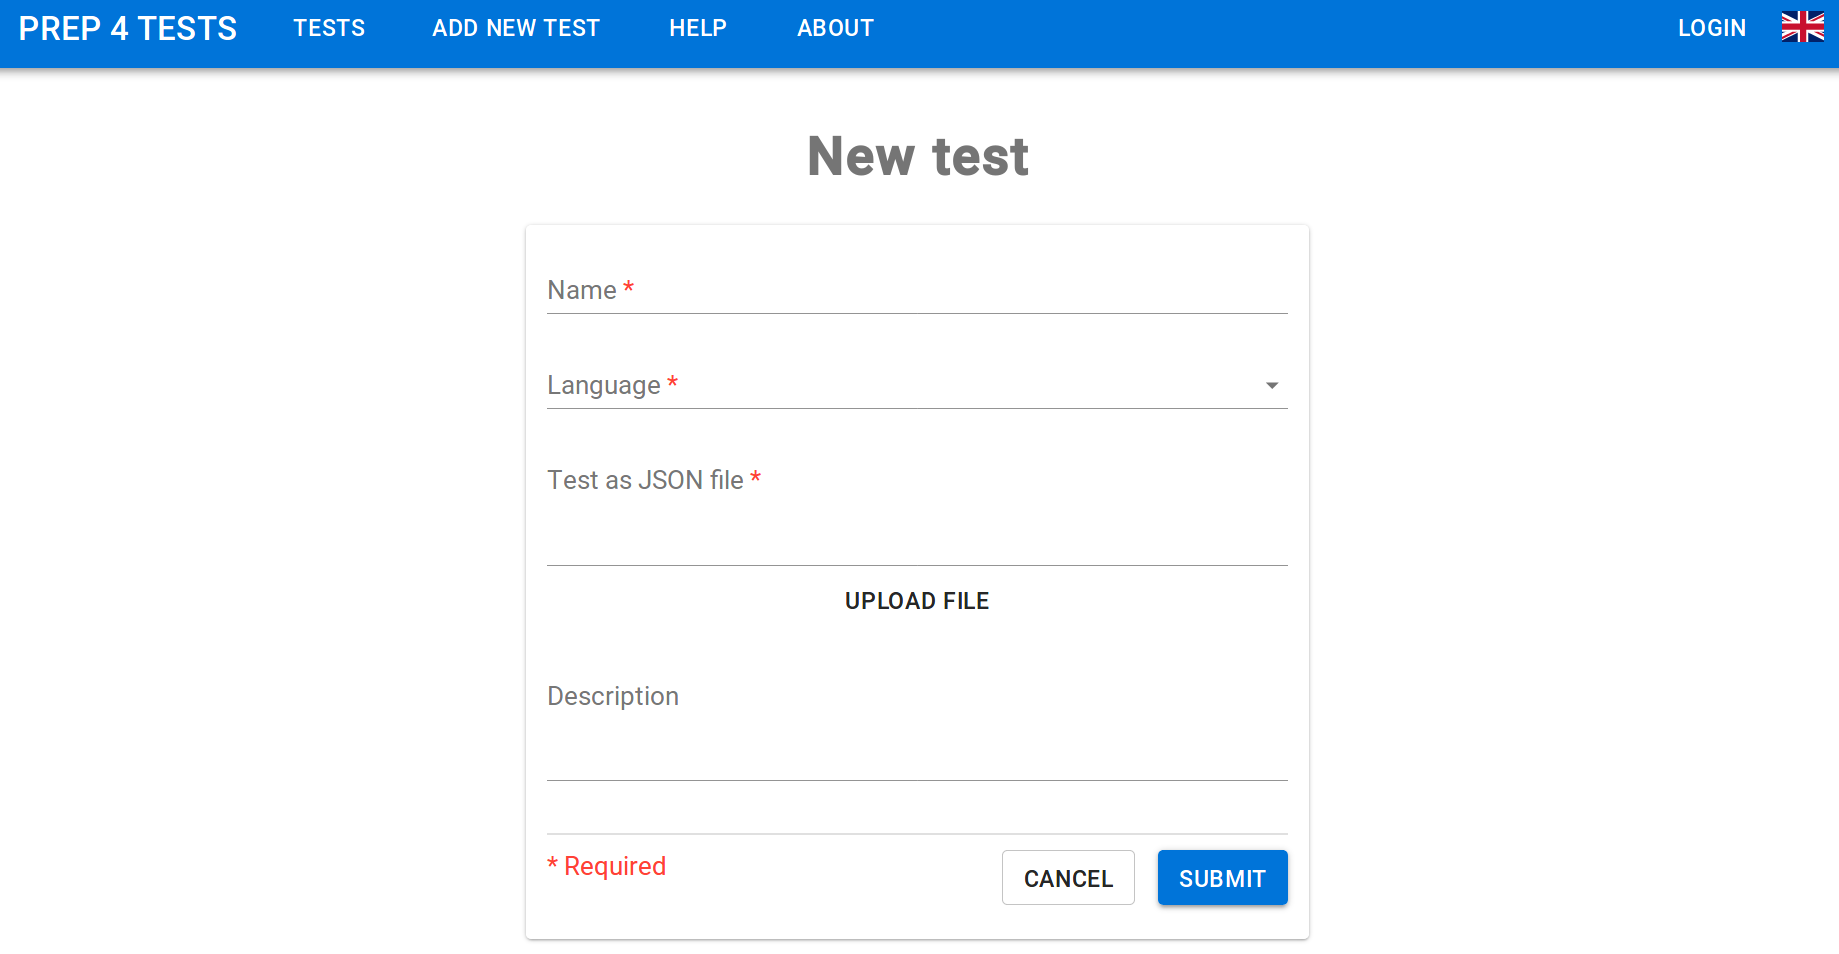
\includegraphics[width=0.75\textwidth,height=0.75\textheight,keepaspectratio]{img/application/example5.png}}
        \caption{add a new test}
      \end{figure}
    \end{frame}

    \begin{frame}{Example 7}
      \begin{figure}
        \fcolorbox{imageBorderColor}{white}{
\includegraphics[width=\textwidth,height=\textheight,keepaspectratio]{img/application/example6.png}}
        \caption{language selection}
      \end{figure}
    \end{frame}

    \begin{frame}{Example 8}
      \begin{figure}
        \fcolorbox{imageBorderColor}{white}{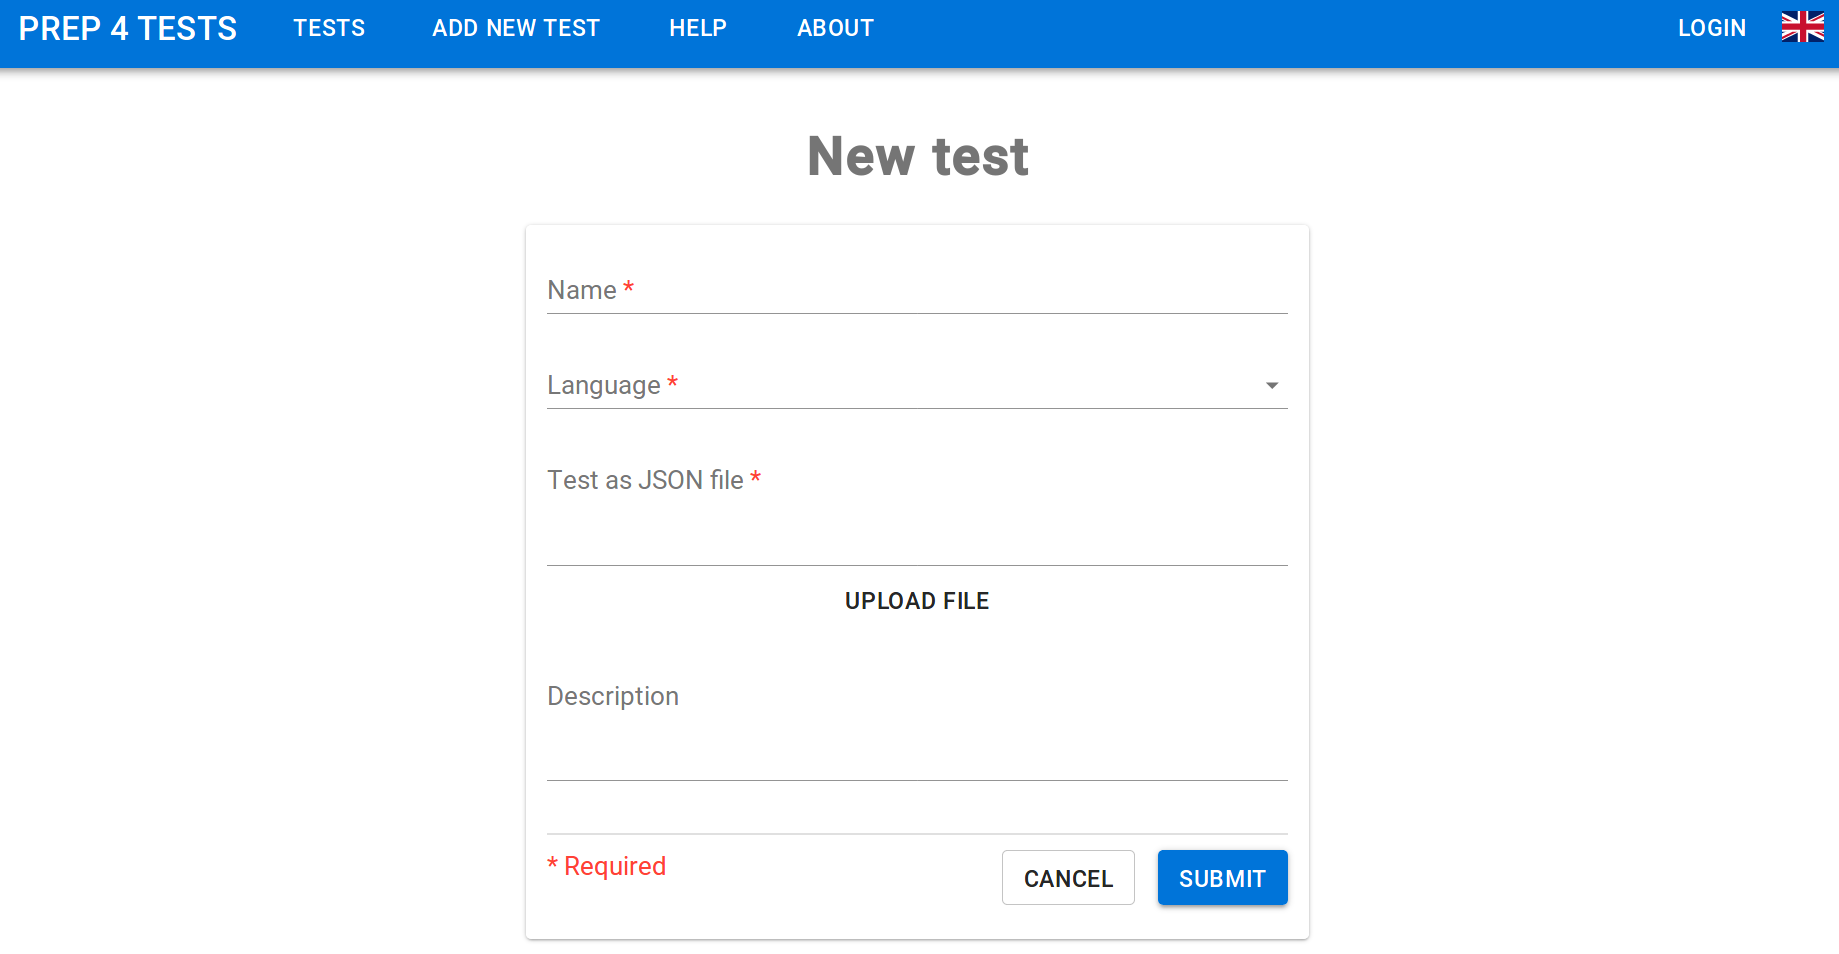
\includegraphics[width=\textwidth,height=\textheight,keepaspectratio]{img/application/example7.png}}
        \caption{help}
      \end{figure}
    \end{frame}

    \begin{frame}{Example 9}
      \begin{figure}
        \fcolorbox{imageBorderColor}{white}{
\includegraphics[width=\textwidth,height=\textheight,keepaspectratio]{img/application/example8.png}}
        \caption{about}
      \end{figure}
    \end{frame}


%##############################################################################

\begin{frame}[plain]
  \vspace{20mm}
  \centerline{Thank you for your attention!}
\end{frame}

\end{document}
